\chapter{Results}
All implemented methods were applied to three scenarios:
\begin{enumerate}
    \item Spiral galaxy simulation (\autoref{sec:galaxy-model}),
    \item Globular cluster simulation (\autoref{sec:globular-cluster-model}),
    \item Galaxy collision simulation (two galaxies modelled as ``disks with holes'', \autoref{subsec:disk-with-hole}).
\end{enumerate}
The choice of these scenarios well illustrates the versatility of the the methods introduced over the last couple of sections.

\section{Spiral galaxy simulation}\label{sec:spiral-galaxy-sim}
The parameters used in the simulation of a spiral galaxy are shown in \autoref{tab:galaxy-parameters}.
\begin{table}[htp]
    \centering
    \caption{Galaxy model parameters used in the simulation.}
    \label{tab:galaxy-parameters}
    \begin{tabular}{lc}
        \toprule
        \textbf{Parameter}   & \textbf{Value}           \\
        \midrule
        Halo radius          & 3 kpc                    \\
        Halo mass            & $60 \times 10^9 M_\odot$ \\
        Disk radius          & 15 kpc                   \\
        Disk mass            & $15 \times 10^9 M_\odot$ \\
        Disk thickness       & 0.3 kpc                  \\
        Disk density profile & Uniformly decreasing     \\
        \bottomrule
    \end{tabular}
\end{table}
The galaxy is simulated as an isolated system; however, in deriving \autoref{eq:poisson-fourier-product}, periodic boundary conditions were assumed.
The simplest way (and the one used) to obtain a free-space solution from the PM method is to extend the computational domain twice in every dimension and fill the space unused in mass distribution with zeros.
The total size of the potential mesh used was $128 \times 128 \times 64$ with the region of interest occupying a box of size $60\, \text{kpc}\times 60\, \text{kpc}\times 30\, \text{kpc}$ located in a $64 \times 64 \times 32$ octant of the mesh.

\subsection{PM method}
In the PM method, $N=50{,}000$ particles were used.
Cell size $H$ and timestep length were set to $60/64=0.9375$ kpc and 1 Myr, respectively.
For convenience, the full configuration of the PM method is presented in \autoref{tab:pm-method-parameters}.
\begin{table}[htp]
    \centering
    \caption{PM method configuration.}
    \label{tab:pm-method-parameters}
    \begin{tabular}{lc}
        \toprule
        \textbf{Parameter}      & \textbf{Value}                     \\
        \midrule
        Effective mesh size     & $64 \times 64 \times 32$           \\
        $H$ (cell size)         & $60/64=0.9375$ kpc                 \\
        DT (time step)          & $1$ Myr                            \\
        Mass assignment scheme  & TSC                                \\
        Finite difference       & Two-point                          \\
        Green's function        & Derived from discretized Laplacian \\
        Time integration method & Leapfrog                           \\
        Number of particles     & 50,000                             \\
        \bottomrule
    \end{tabular}
\end{table}
The system's evolution over 200 Myr is shown in \autoref{fig:spiral-galaxy-evolution-pm}.

\begin{figure}[!ht]
    \centering
    \begin{subfigure}[b]{0.45\textwidth}
        \centering
        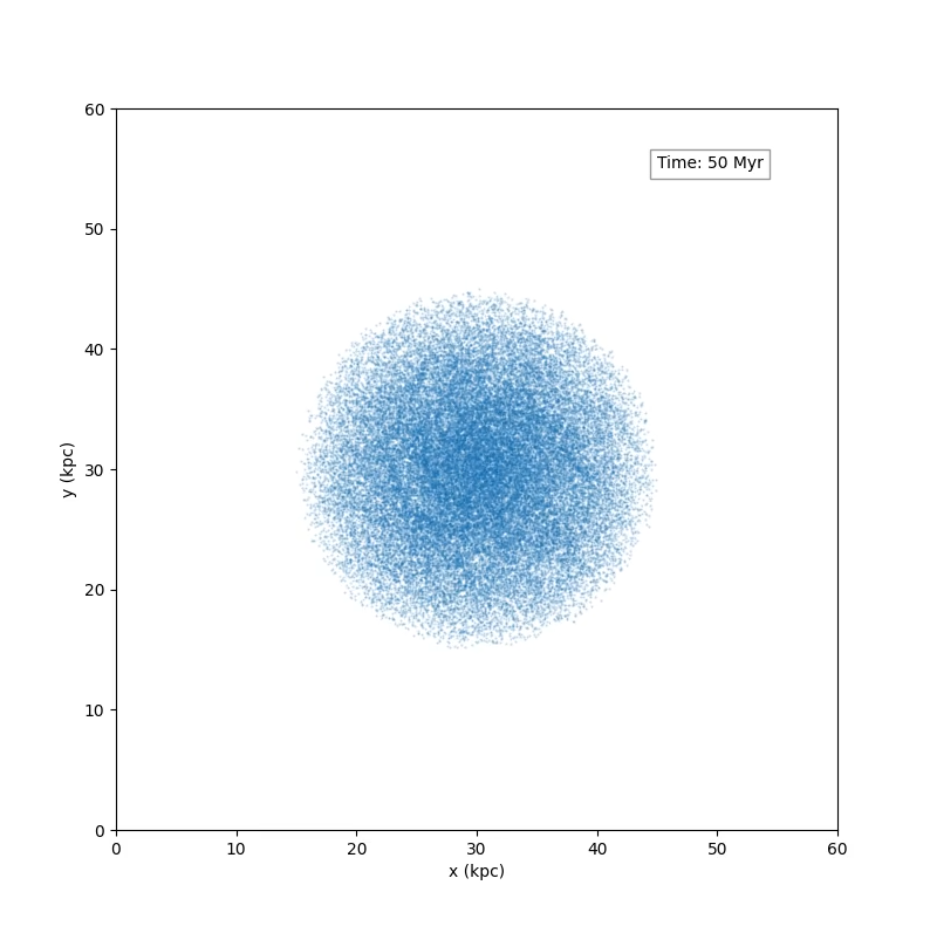
\includegraphics[width=\textwidth]{chapters/results/img/pm-galaxy/50myr.png}
        \caption{$t=50\,\text{Myr}$}
        \label{fig:spiral-galaxy-evolution-pm-sub1}
    \end{subfigure}
    \hfill
    \begin{subfigure}[b]{0.45\textwidth}
        \centering
        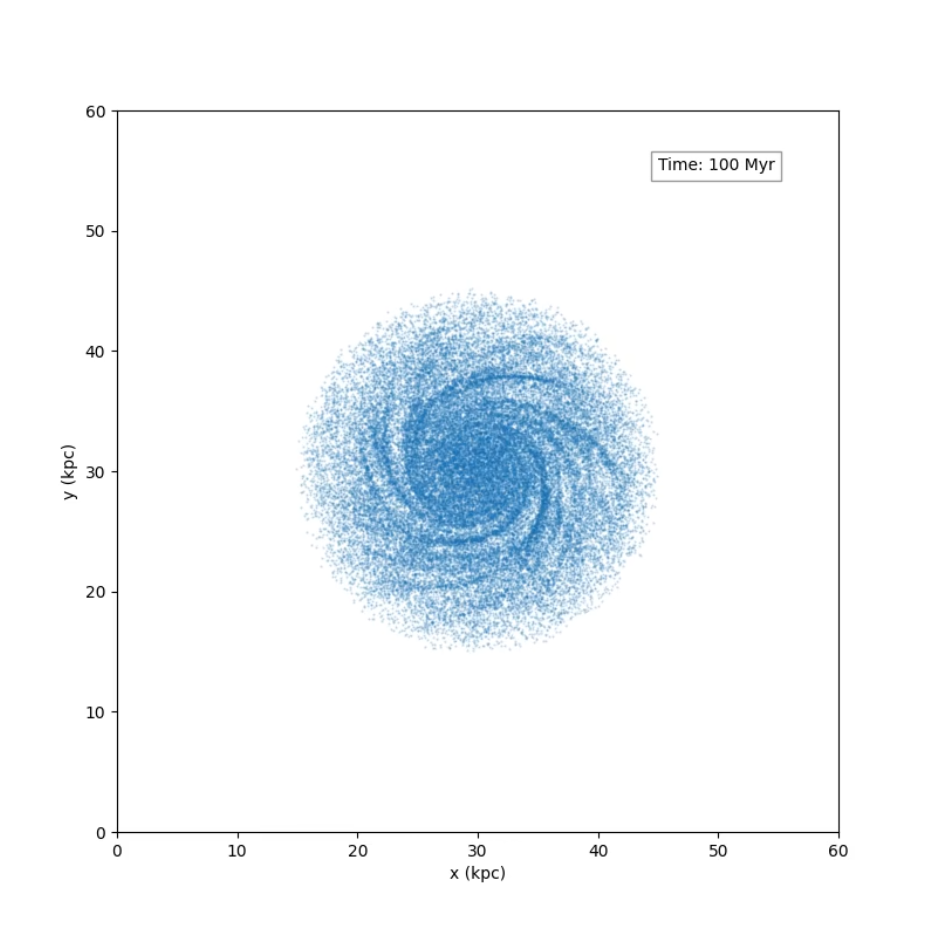
\includegraphics[width=\textwidth]{chapters/results/img/pm-galaxy/100myr.png}
        \caption{$t=100\,\text{Myr}$}
        \label{fig:spiral-galaxy-evolution-pm-sub2}
    \end{subfigure}

    \vspace{0.2cm}

    \begin{subfigure}[b]{0.45\textwidth}
        \centering
        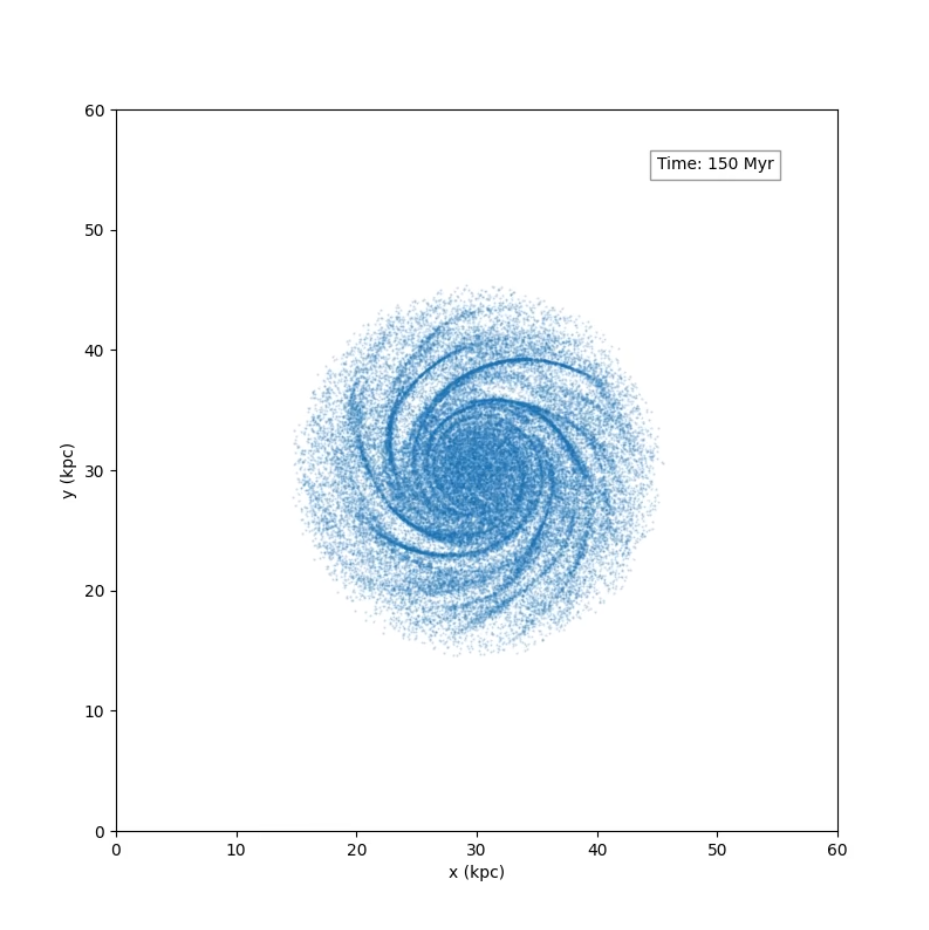
\includegraphics[width=\textwidth]{chapters/results/img/pm-galaxy/150myr.png}
        \caption{$t=150\,\text{Myr}$}
        \label{fig:spiral-galaxy-evolution-pm-sub3}
    \end{subfigure}
    \hfill
    \begin{subfigure}[b]{0.45\textwidth}
        \centering
        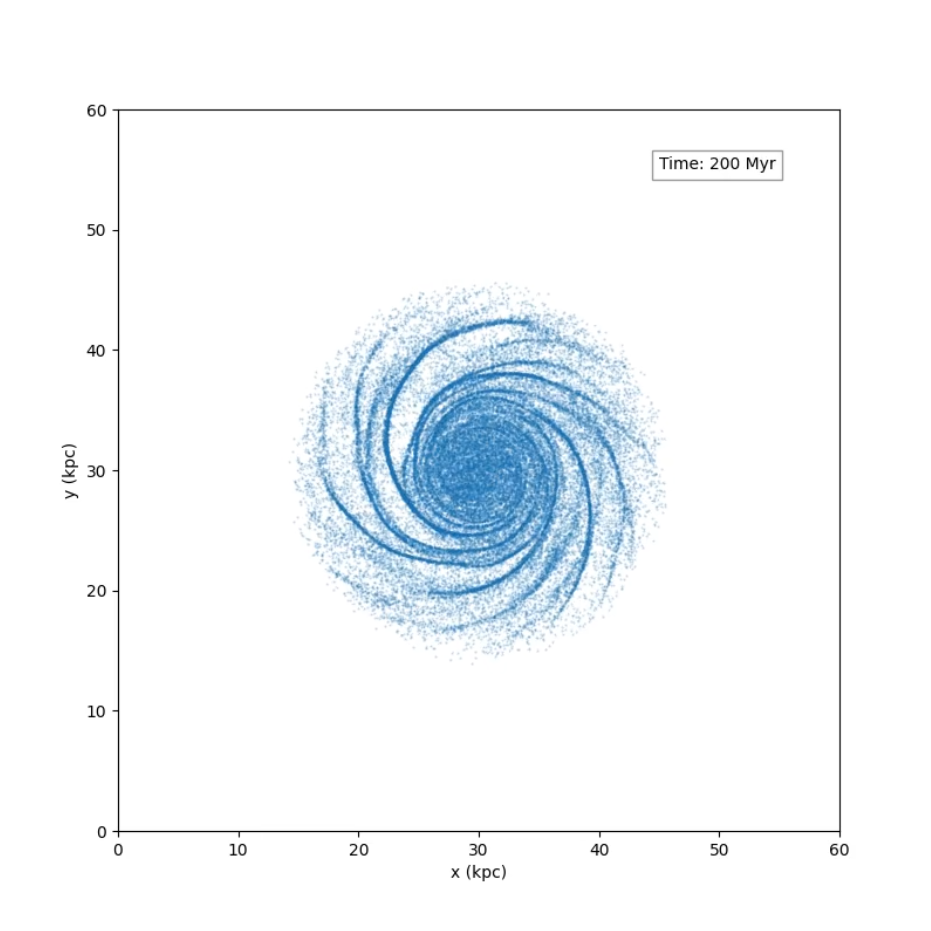
\includegraphics[width=\textwidth]{chapters/results/img/pm-galaxy/200myr.png}
        \caption{$t=200\,\text{Myr}$}
        \label{fig:spiral-galaxy-evolution-pm-sub4}
    \end{subfigure}

    \caption{Evolution of a spiral galaxy as predicted by the PM method.}
    \label{fig:spiral-galaxy-evolution-pm}
\end{figure}

During the simulation, total energy $E = \textrm{KE} + \textrm{PE}$, angular momentum $\mathbf{l}$, and the $z$-component of the momentum vector $\mathbf{p}$ should stay constant.
The $x$- and $y$-components of momentum change due to the presence of an external gravitational field (representing the halo) that exerts force $\mathbf{F}^\text{ext}$ on the system.
We can verify if this variation satisfies the expected relation
\begin{equation}\label{eq:expected-momentum-change}
    \dot{\mathbf{p}} = \mathbf{F}^\text{ext}
\end{equation}
by finding the initial total momentum $\mathbf{p}(t = 0)$ and incrementing the value of $\mathbf{p}$ in each time-step by $\mathbf{F}^\text{ext}\textrm{DT}$.

The exact calculation of the potential energy \cite{taylor2005classical} using the formula
\begin{equation*}
    \textrm{PE} = -\sum_{i=1}^{N}\sum_{j=i+1}^{N}\frac{G m_i m_j}{r_{ij}}
\end{equation*}
is computationally infeasible considering the $O(N^2)$ cost.
An approximation based on the potential values at mesh points,
\begin{equation*}
    \textrm{PE} \approx \frac{V}{2}\sum_{\mathbf{p}} \rho(\mathbf{x}_\mathbf{p})\phi(\mathbf{x}_\mathbf{p}),
\end{equation*}
is used instead (for derivation, refer to \cite{Hockney1988}).
\begin{figure}[!ht]
    \centering
    \begin{subfigure}[b]{0.45\textwidth}
        \centering
        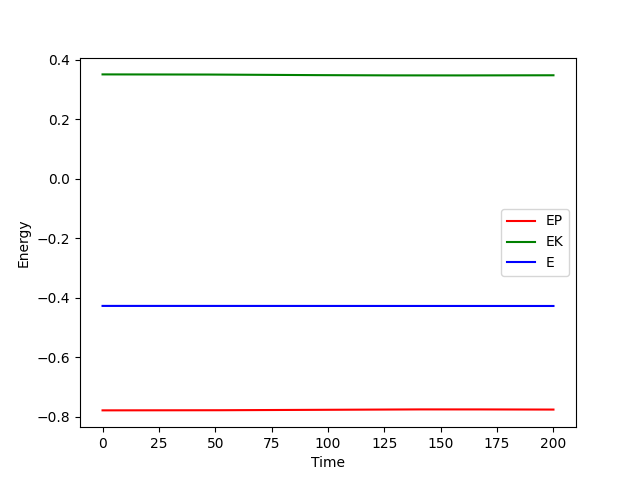
\includegraphics[width=\textwidth]{chapters/results/img/pm-galaxy/energy.png}
        \caption{Energy}
        \label{fig:physical-quantities-pm-sub1}
    \end{subfigure}
    \hfill
    \begin{subfigure}[b]{0.45\textwidth}
        \centering
        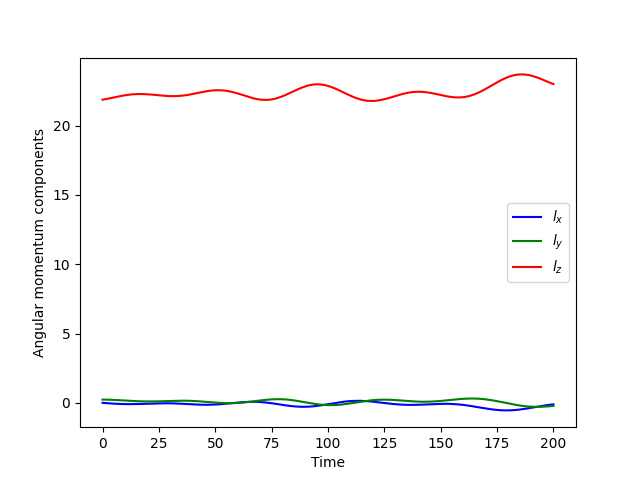
\includegraphics[width=\textwidth]{chapters/results/img/pm-galaxy/angular-momentum.png}
        \caption{Angular momentum}
        \label{fig:physical-quantities-pm-sub2}
    \end{subfigure}

    \vspace{0.2cm}

    \begin{subfigure}[b]{0.45\textwidth}
        \centering
        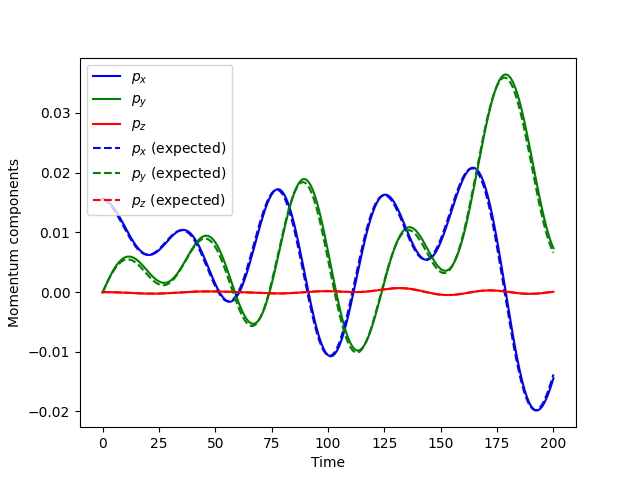
\includegraphics[width=\textwidth]{chapters/results/img/pm-galaxy/momentum.png}
        \caption{Momentum; broken lines represent the expected momentum following \autoref{eq:expected-momentum-change}}
        \label{fig:physical-quantities-pm-sub3}
    \end{subfigure}

    \caption{Fundamental physical quantities describing the system over time in the PM simulation.
        Time is in Myr, and the quantities are expressed in units consistent with \autoref{tab:galaxy-parameters}}
    \label{fig:physical-quantities-pm}
\end{figure}

\subsection{\texorpdfstring{\PThreeM{}}{P3M} method}
The \PThreeM{}-based simulation uses the same parameters as the PM method.
The reference force was calculated using the $S_1$ shape formula (\autoref{eq:s1-reference-force}) with particle diameter $a=3H$.
The cutoff radius was set to $r_e=0.7a$.
One extra free parameter is the \textit{softening length} $\epsilon$, which modifies the universal law of gravitation so that division by zero can be avoided, i.e., the modified law is
\begin{equation*}
    F^\text{soft}_{ij}(r) = \frac{G m_i m_j}{r_{ij}^2 + \epsilon^2}.
\end{equation*}
In the simulation, $\epsilon$ was set arbitrarily to $1.5$ kpc.
The whole configuration of the \PThreeM{} method is conveniently shown in \autoref{tab:p3m-method-parameters}.
The system's evolution is presented in \autoref{fig:spiral-galaxy-evolution-p3m}, and the graphs of energy, angular momentum, and momentum components vs. time are shown in \autoref{fig:physical-quantities-p3m}.

\subsection{Barnes-Hut algorithm}
For the Barnes-Hut algorithm test, the initial conditions of the system remain the same as in the two previous simulations.
The softening length $\epsilon$ was set to 1 kpc, and quadrupole terms were omitted.
The whole configuration of the method is shown in \autoref{tab:bh-method-parameters}.
The snapshots of the simulation are displayed in \autoref{fig:spiral-galaxy-evolution-bh}, and the graphs showing how the energy, momentum, and angular momentum varied over time are shown in \autoref{fig:physical-quantities-bh}.

\subsection{Commentary}
All of the implemented methods successfully reproduced the expected structural features of a spiral galaxy.
A region of high density is clearly localized in the center of the galaxy, and characteristic spiral arms emerge around the 150 Myr mark.
The snapshots from all three simulations (\autoref{fig:spiral-galaxy-evolution-pm}, \autoref{fig:spiral-galaxy-evolution-p3m}, and \autoref{fig:spiral-galaxy-evolution-bh}) show similar evolution of the system over time, with the last snapshot of each simulation visually resembling a real-world spiral galaxy (cf. \autoref{fig:ngc-628}).
It is worth noting, however, that the system evolves more rapidly in the PM-based simulation.
For instance, the spiral arms are significantly more developed at $t = 100$ Myr (\autoref{fig:spiral-galaxy-evolution-pm-sub2}) compared to the same time point in the simulations using the other two methods.
This accelerated evolution is likely due to the smaller ``induced softening length'' inherent to the PM method, which results in stronger gravitational forces. These limitations were anticipated and discussed in \autoref{subsubsec:pm-global-picture}.

Energy plots (\autoref{fig:physical-quantities-pm-sub1}, \autoref{fig:physical-quantities-p3m-sub1}, and \autoref{fig:physical-quantities-bh-sub1}) show that each of the methods tested conserved the total energy.
The plots of angular momentum over time (\autoref{fig:physical-quantities-pm-sub2}, \autoref{fig:physical-quantities-p3m-sub2}, and \autoref{fig:physical-quantities-bh-sub2}) illustrate that the angular momentum was \textit{on average} constant with the variations stemming from the presence of the external halo field.
Finally, the momentum plots (\autoref{fig:physical-quantities-pm-sub3}, \autoref{fig:physical-quantities-p3m-sub3}, and \autoref{fig:physical-quantities-bh-sub3}) demonstrate that the $z$-component of the momentum vector remains constant, while the remaining components change (again due to the external field).
The comparison of the actual values of the momentum with the theoretical values, updated in each timestep according to \autoref{eq:expected-momentum-change}, shows that the change in the $x$- and $y$-components is correct.

\section{Globular cluster simulation}
The globular cluster is simulated using the Plummer model with parameters set to the values in \autoref{tab:cluster-parameters}.
\begin{table}[htp]
    \centering
    \begin{tabular}{|l|c|}
        \hline
        \textbf{Parameter} & \textbf{Value}          \\
        \hline
        $a$ (spread)       & 2 pc                    \\
        Mass               & $1 \times 10^6 M_\odot$ \\
        Maximum radius     & 15 pc                   \\
        \hline
    \end{tabular}
    \caption{Galaxy model parameters used in the simulation.}
    \label{tab:cluster-parameters}
\end{table}
The \textit{maximum radius} parameter was introduced simply to confine the cluster to a predefined computational domain.
We restrict the presentation of our results to the simulation conducted using the Barnes-Hut algorithm, since other methods yielded very similar results.

\subsection{Barnes-Hut algorithm}
The configuration of the Barnes-Hut algorithm used in the globular cluster simulation is given in \autoref{tab:bh-method-parameters-cluster}.
\begin{table}[htp]
    \centering
    \begin{tabular}{|l|c|}
        \hline
        \textbf{Parameter}            & \textbf{Value} \\
        \hline
        $\theta$ (opening angle)      & 0.5            \\
        $\epsilon$ (softening length) & 0.5 pc         \\
        DT (time step)                & $1$ kyr        \\
        Highest multipole term        & quadrupole     \\
        \hline
    \end{tabular}
    \caption{Barnes-Hut method configuration.}
    \label{tab:bh-method-parameters-cluster}
\end{table}
The conservation of energy, momentum, and angular momentum during the simulation is demonstrated in \autoref{fig:physical-quantities-bh-cluster}.
\begin{figure}[htp]
    \centering
    \begin{subfigure}[b]{0.45\textwidth}
        \centering
        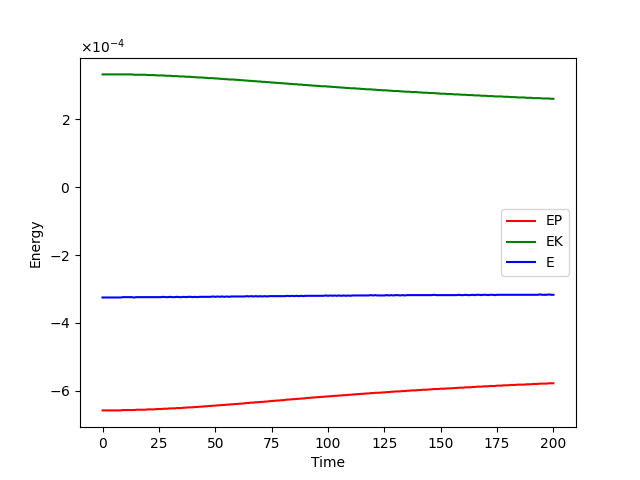
\includegraphics[width=\textwidth]{img/bh-cluster/energy.png}
        \caption{Energy}
        \label{fig:physical-quantities-bh-cluster-sub1}
    \end{subfigure}
    \hfill
    \begin{subfigure}[b]{0.45\textwidth}
        \centering
        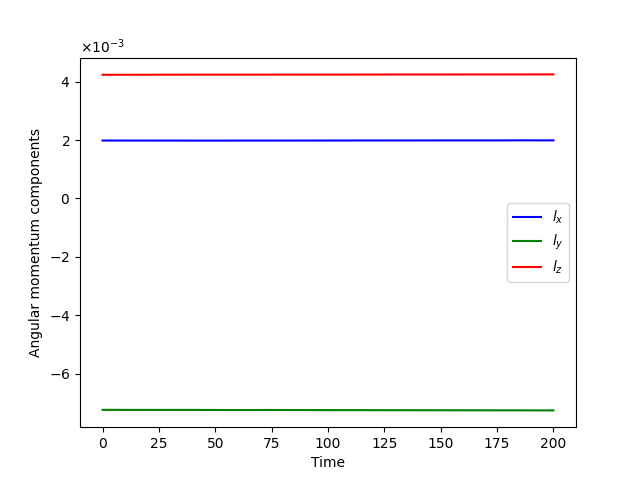
\includegraphics[width=\textwidth]{img/bh-cluster/angular-momentum.png}
        \caption{Angular momentum}
        \label{fig:physical-quantities-bh-cluster-sub2}
    \end{subfigure}

    \vspace{0.5cm}

    \begin{subfigure}[b]{0.45\textwidth}
        \centering
        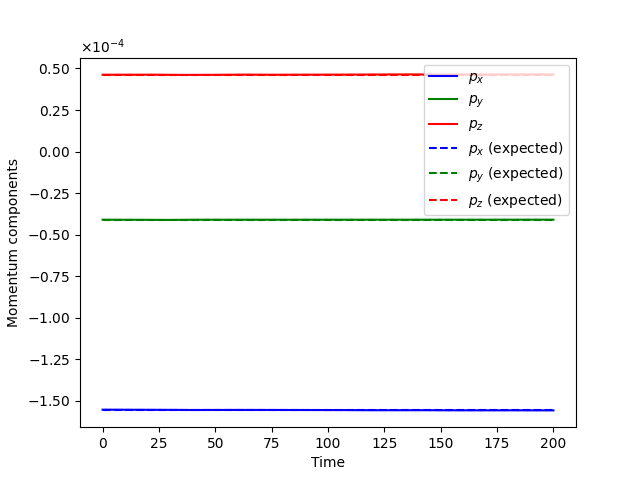
\includegraphics[width=\textwidth]{img/bh-cluster/momentum.png}
        \caption{Momentum; broken lines represent the expected momentum following \autoref{eq:expected-momentum-change}}
        \label{fig:physical-quantities-bh-cluster-sub3}
    \end{subfigure}

    \caption{Fundamental physical quantities describing the system over time in the Barnes-Hut algorithm.
        Time is in kyr and the quantities are expressed in units consistent with \autoref{tab:cluster-parameters}}
    \label{fig:physical-quantities-bh-cluster}
\end{figure}
Notice that the conservation of momentum and angular momentum is possible due to a lack of any external forces (this is contrasted with the previous test -- galaxy simulation with halo modelled a fixed, external field).
The evolution of the system (initial positions and after 200 kyr) is shown in \autoref{fig:cluster-evolution-bh}.
\begin{figure}[htp]
    \centering
    \begin{subfigure}[b]{0.45\textwidth}
        \centering
        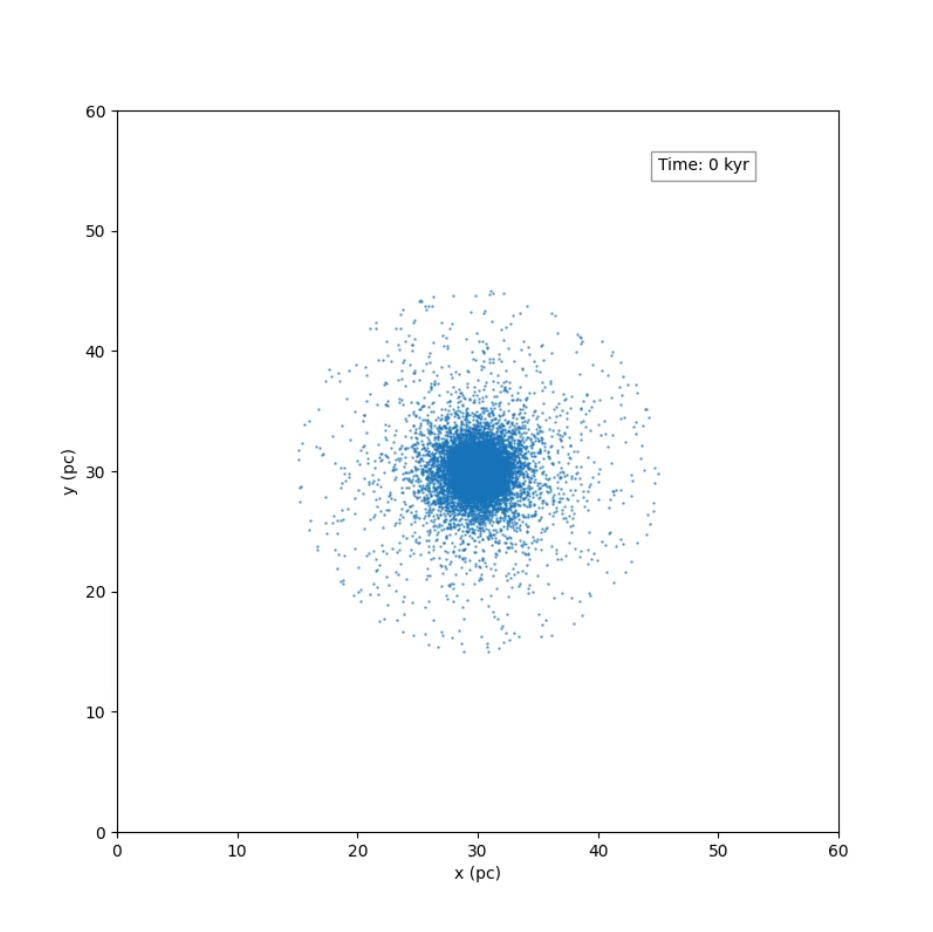
\includegraphics[width=\textwidth]{img/bh-cluster/0kyr.png}
        \caption{$t=0\,\text{kyr}$}
        \label{fig:cluster-evolution-bh-cluster-sub1}
    \end{subfigure}
    \hfill
    \begin{subfigure}[b]{0.45\textwidth}
        \centering
        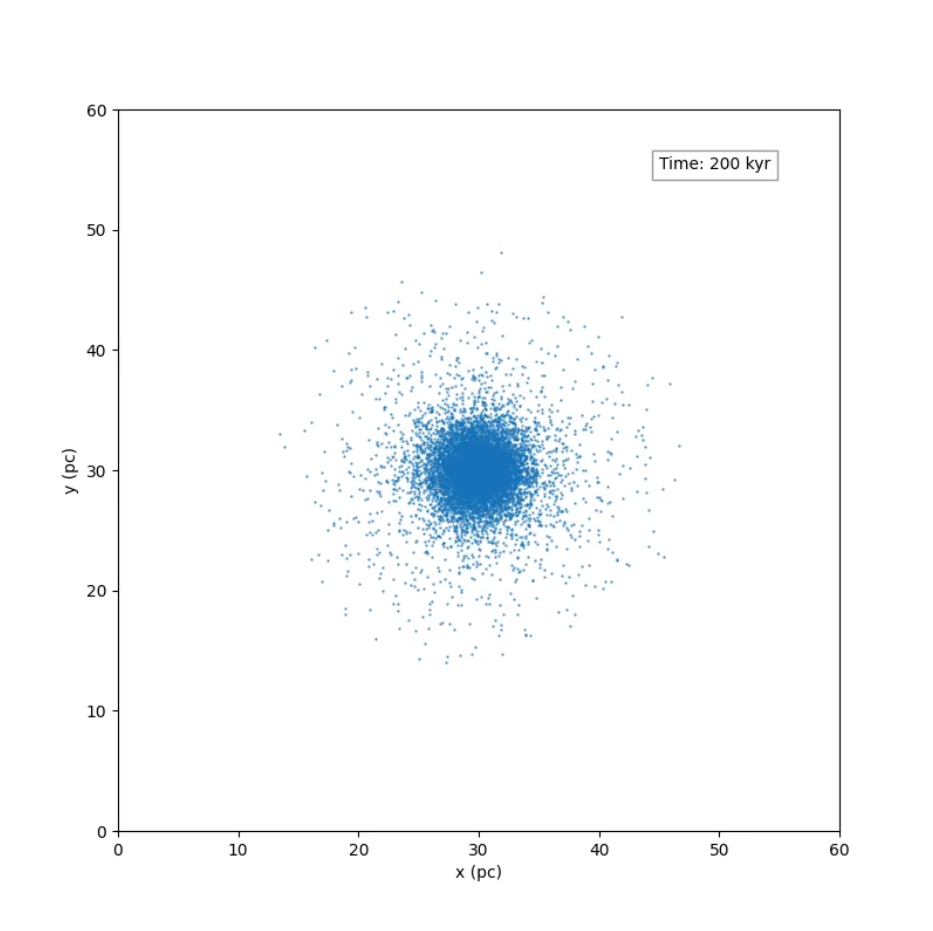
\includegraphics[width=\textwidth]{img/bh-cluster/200kyr.png}
        \caption{$t=200\,\text{kyr}$}
        \label{fig:cluster-evolution-bh-cluster-sub2}
    \end{subfigure}
    \caption{Evolution of a globular cluster as predicted by the Barnes-Hut algorithm.}
    \label{fig:cluster-evolution-bh}
\end{figure}
As can be seen, the system remains stable and bound gravitationally.
Also, in the initial snapshot (\autoref{fig:cluster-evolution-bh-cluster-sub1}) the effect of restricting the sampled points to a sphere of radius can be seen.
The system bears general resemblance to real-world globular clusters (cf. \autoref{fig:messier-13}).
\section{Galaxy collision simulation}
We conclude showcasing the applications of our program with a simulation of collision of two galaxies.
The parameters describing the galaxies are given in \autoref{tab:galaxy-parameters-collision}.
\begin{table}[htp]
    \centering
    \begin{tabular}{|l|c|c|}
        \hline
        \textbf{Parameter}   & \textbf{Galaxy 1}        & \textbf{Galaxy 2}        \\
        \hline
        Center position      & (40, 30, 15) kpc         & (80, 30, 15) kpc         \\
        Halo radius          & 3 kpc                    & 2 kpc                    \\
        Halo mass            & $60 \times 10^9 M_\odot$ & $40 \times 10^9 M_\odot$ \\
        Disk radius          & 15 kpc                   & 10 kpc                   \\
        Disk mass            & $15 \times 10^9 M_\odot$ & $10 \times 10^9 M_\odot$ \\
        Disk thickness       & 0.3 kpc                  & 0.3 kpc                  \\
        Disk density profile & Uniformly decreasing     & Uniformly decreasing     \\
        Number of particles  & $3 \times 10^4$          & $3 \times 10^4$          \\
        \hline
    \end{tabular}
    \caption{Galaxy model parameters used in the simulation.}
    \label{tab:galaxy-parameters-collision}
\end{table}
\subsection{Barnes-Hut algorithm}
The configuration of the algorithm is given in \autoref{tab:bh-method-parameters-collision}.
\begin{table}[htp]
    \centering
    \begin{tabular}{|l|c|}
        \hline
        \textbf{Parameter}            & \textbf{Value} \\
        \hline
        $\theta$ (opening angle)      & 1              \\
        $\epsilon$ (softening length) & 1.3 kpc        \\
        DT (time step)                & $1$ Myr        \\
        Simulation duration           & 400 Myr        \\
        Highest multipole term        & Monopole       \\
        \hline
    \end{tabular}
    \caption{Barnes-Hut method configuration.}
    \label{tab:bh-method-parameters-collision}
\end{table}


\section{Performance analysis}
The performance analysis was conducted in the setting of the spiral galaxy simulation on a computer equipped with an Intel Core i7-9750H CPU (2.60GHz) and an NVIDIA GeForce GTX 1650 GPU.
By that, we mean that not only the particle distribution was the same as in \autoref{sec:spiral-galaxy-sim}, but also the configuration of the algorithms remained unchanged.
Moreover, to obtain results that most closely correspond to a real scenario of using the program, diagnostic information collection was enabled, and the simulation state was saved after each frame.
The diagnostic information mentioned here refers collectively to energy (kinetic, potential, and total), momentum, and angular momentum.
It is essential to keep in mind that in the case of the PM and \PThreeM{} methods, recording these quantities comes with an additional overhead of converting the state of the system from code to ``original'' units.
Potentially, suitable code units could also be introduced in the case of the Barnes-Hut algorithm, but we did not find this necessary.
Saving the state of the system in each frame also incurs additional overhead related to disk I/O operations.
In our implementation, the output is buffered so that data is written to disk at a reasonable frequency.
We also note that the reported running time is averaged over 100 iterations.

\begin{figure}[!ht]
    \centering
    \begin{subfigure}[b]{0.48\textwidth}
        \centering
        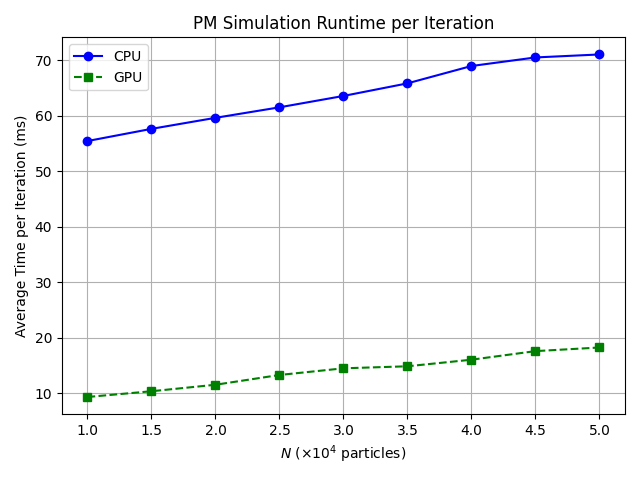
\includegraphics[width=\linewidth]{chapters/results/img/perf/pm_time.png}
        \caption{PM method}
        \label{fig:pm-running-time}
    \end{subfigure}
    \hfill
    \begin{subfigure}[b]{0.48\textwidth}
        \centering
        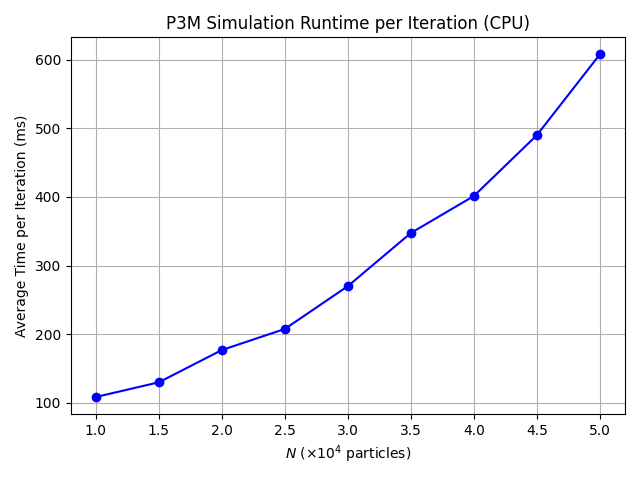
\includegraphics[width=\linewidth]{chapters/results/img/perf/p3m_time.png}
        \caption{\PThreeM{} method}
        \label{fig:p3m-running-time}
    \end{subfigure}

    \vspace{1em}

    \begin{subfigure}[b]{0.48\textwidth}
        \centering
        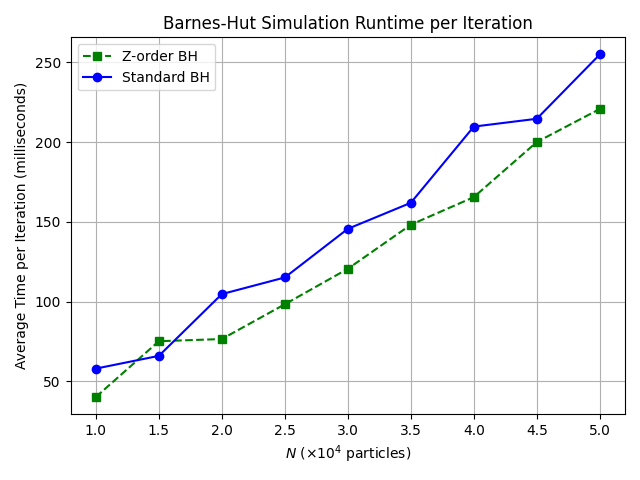
\includegraphics[width=\linewidth]{chapters/results/img/perf/bh_time.png}
        \caption{Barnes-Hut algorithm}
        \label{fig:bh-running-time}
    \end{subfigure}

    \caption{Running time of the different methods as a function of the number of particles.}
    \label{fig:method-running-time-comparison}
\end{figure}

The running time for the PM method is shown in \autoref{fig:method-running-time-comparison}.
The GPU implementation provides, at best, a five-fold speedup over the CPU implementation.
This is in stark contrast with the results reported in \autoref{subsec:gpu-variant} (1200\% speedup).
The difference between the two results stems from the fact in \autoref{subsec:gpu-variant}, we considered an ``idealized scenario'' where the data transfers from device to host and disk I/O operations were reduced to the absolute minimum, saving only the \textit{final state} of the simulation.
Both plots (GPU and CPU variants) exhibit linear time dependence as expected.

The \PThreeM{} method comes out as the least performant method among these considered in the thesis.
The runtime per iteration was up to 8.5 times longer than the CPU variant of the PM method and up to 3.5 times longer than the Barnes-Hut algorithm in its standard variant.
Moreover, it is apparent that the algorithm does not scale linearly.
Indeed, the behavior is well described by a quadratic function with a leading coefficient of 21.3 ms.
As we pointed out in \autoref{subsec:p3m-error-analysis}, the influence of the $O(N^2)$ direct summation part of the algorithm can reduced at the expense of weaker accuracy.

The Barnes-Hut algorithm was timed in two configurations: with the standard tree construction and the improved one (introduced in \autoref{sec:accelerating-tree-construction}).
The range of $ N $ considered in the test is too small to reveal the linearithmic runtime dependence on $ N $ fully.
In any case, the Barnes-Hut algorithm comes second in the comparison, with running times 3.5 slower than the PM method in the standard variant and only 3.2 times slower if the improved tree construction is used.
We note that a comparison with \autoref{fig:z-order-tree-time} reveals that the tree construction is responsible for around 15\% of the total running time of the simulation.

% \subsection{Performance analysis}
% The PM and \PThreeM{} methods were implemented exactly as described in the previous sections.
% The PM method was developed for both CPU and GPU architectures, using C++ and CUDA C++, respectively.
% The implementation relies on external libraries for fast Fourier transform computations: FFTW for the CPU version and cuFFT for the GPU version.
% A performance comparison of the PM method was conducted with $N$ ranging between 50,000 and 1,000,000 over 200 iterations (TSC mass assignment and two-point finite difference).
% The tests were run on a system equipped with an Intel(R) Core(TM) i7-9750H CPU @ 2.60GHz and an NVIDIA GeForce GTX 1650 GPU.
% For the purposes of performance evaluation, the parts of the code responsible for diagnostics collection (energy, momentum, etc.) were switched off.
% Since disk IO (saving simulation state) was the most time-consuming part of both the CPU and GPU implementation, only the final state of the simulation was saved in these tests.
% This means that data transfers from device to host were also not taken into account.
% The results of the test are displayed in \autoref{fig:cpu-vs-gpu-pm}.


% For the \PThreeM{} method, performance was measured using $N=50,000$ particles on a $128 \times 128 \times 64$ mesh with the TSC assignment scheme.
% The total runtime was approximately 1 minute and 30 seconds, with the time distribution among key algorithm components as follows:
% \begin{itemize}
%     \item HOC table initialization: 12\%
%     \item Short-range force calculations: 80\%
%     \item PM step: 7.5\%
% \end{itemize}
% The code is available at \url{https://github.com/AleksyBalazinski/ParticleSimulation} under the MIT license.